%
% A (non-exhaustive) list of TODOs:
%


\chapter{PhoG: Photon Gun}\label{chapter:phog}
Goal of chapter: analyse and model the PhoG device and its efficacy for producing, from a classical input, (i) bright sub-Poissonian state; (ii) entangled state


\section{Introduction}
\begin{itemize}
\item Introduce dissipation as a means for state engineering
\item Introduce our goal to produce single-photons (or close to single-photons)
\item Introduce this chapter, include a chapter outline, and provide motivation for why we will look at different models
\end{itemize}

\begin{figure}[htp]
\centering
\includegraphics[draft=false, width=\linewidth]{phog/phog_models}
\caption{\label{fig:phog_models} Hierarchy of models of the phog device, from least realistic (left) to most realistic (right). We will discuss each model in turn throughout the rest of this chapter. \MakeUppercase{\romannumeral 1}: Single-mode model. \MakeUppercase{\romannumeral 2}: Two-mode model. \MakeUppercase{\romannumeral 3}: Three-mode model. \MakeUppercase{\romannumeral 4}: Multi-mode model. \MakeUppercase{\romannumeral 5} Multi-mode model embedded in glass. }
\end{figure}

\section{Single-mode model}

\begin{figure}[htp]
\centering
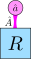
\includegraphics[width=0.2\linewidth, draft=false]{phog/single_mode}
\caption{\label{fig:phog_single_mode} A single bosonic mode, $a$, is coupled to a Markovian reservoir $R$ by operator $\hat{A}$. }
\end{figure}


Consider the model displayed in Fig.~\ref{fig:phog_single_mode} (c.f. Fig.~\ref{fig:phog_models}\MakeUppercase{\romannumeral 1}), which consists of a single bosonic mode, $a$, coupled to a reservoir $R$ via a reservoir operator $\mathcal{A}$. The annihilation (creation) operator for mode $a$ is denoted $\hat{a} \left(\hat{a}^\dagger\right)$, and the density matrix containing all information about the state of the mode is denoted $\rho_a$. This model will prove illustrative of several principles which we will develop throughout the chapter. Assuming that reservoir $R$ is Markovian, the evolution of mode $a$ is given by the following quantum master equation in Lindblad form\footnote{Equations in this form will be referred to as ``Lindblad equations''}

\begin{equation}
\ddt \rho_a = something
\end{equation}



